\documentclass{article}
\usepackage{amsfonts,amssymb,amsthm,amsmath,eucal,tabu,url}
\usepackage{hyperref}
\usepackage[T1]{fontenc}
\usepackage{graphicx}
\usepackage[utf8]{inputenc}
\usepackage{animate}


\theoremstyle{plain}
\newtheorem{thm}{Theorem}[section]
\newtheorem{theorem}[thm]{Theorem}
\newtheorem*{theoremA}{Theorem A}
\newtheorem*{theoremB}{Theorem B}
\newtheorem*{theoremC}{Theorem C}
\newtheorem{lemma}[thm]{Lemma}
\newtheorem{proposition}[thm]{Proposition}
\newtheorem{corollary}[thm]{Corollary}
\newtheorem{conjecture}[thm]{Conjecture}

\theoremstyle{definition}
\newtheorem{definition}[thm]{Definition}
\newtheorem{remark}[thm]{Remark}
\newtheorem{example}[thm]{Example}
\newtheorem{claim}[thm]{Claim}
\newtheorem{question}[thm]{Question}
\newtheorem{problem}[thm]{Problem}
\newtheorem{fact}[thm]{Fact}
\newtheorem*{notation}{Notation}
\newtheorem*{sketch}{Sketch of Proof}

\newtheorem{thevarthm}[thm]{\varthmname}
\newenvironment{varthm}[1]{\def\varthmname{#1}\begin{thevarthm}}{\end{thevarthm}\def\varthmname{}}
\newenvironment{varthm*}[1]{\trivlist\item[]{\bf #1.}\it}{\endtrivlist}



\title{%
  \huge On the shortest Path between two vertices in Permutation Polyope}
\author{Filip Zieliński}
\date{23/04/2024 r.}

\begin{document}
\maketitle
\section{Abstract}
\begin{definition} \label{def2}
    \textbf{Polytope.} The convex hull of a finite set of points in $ \mathbb{R}^d$ is called a \textit{polytope}.
\end{definition}
    Let $c_{1},..., c_{m}$ be vectors from $ \mathbb{R}^d$ and let $\beta_{1}, ... , \beta_{m}$ be real numbers and additionally $\langle \cdot,\cdot \rangle$ be  the standard inner product. The set:
    $$P = \{ x \in \mathbb{R}^d : \langle c_{i},x \rangle \leq \beta_{i},  i=1,..,m\}$$
    is called \textit{polyhedron.}
If polyhedron is bounded it is also a Polytope. 
\begin{definition}
        A \textit{vertex} of polyhedron $P$ is a point $a \in P$ provided that for any two points $b,c \in P$  such that $\frac{b+c}{2} = a$ one must have $b = c = a$.
\end{definition}

\begin{definition}\label{def4}
    \textbf{Doubly stochastic Matrix.} An  $n \times n $  matrix $M=(\alpha_{ij}) $ is called \textit{doubly stochastic} if it is non-negative and the sum of elements in every row and every columns equals 1:
    \begin{enumerate}
        \item $ \sum_{i=1}^{n}\alpha_{ij} =1 $ for $j=1,... ,n$,
        \item $ \sum_{j=1}^{n}\alpha_{ij}=1 $ for $i=1,... ,n$,
        \item $\alpha_{ij} >0$ for $i,j=1,.. ,n$.
    \end{enumerate}
    
\end{definition}
\begin{definition}
    The polyhedron $B_{n}$ of all $n \times n$ doubly stochastic matrices is called the \textit{Birkhoff Polytope}, where  
    we consider  $n \times n $ matrix $X$ as point in $\mathbb{R}^{n^2}$.
\end{definition}
Birkhoff Polyope lies in $(n-1)^2$ dimensional affine subspace of $\mathbb{R}^{n^2}$. \newline 
What's more  \textbf{Birkhoff - von Neumann Theorem} states that the vertices of $B_n$ are exactly permutation matrices. \newline 
Now let consider a point $x \in \mathbb{R}^n$. We define a $\textit{Permutation Polytope}$ $P(x)$ to be a convex hull of all possible permutations of coordinates of  point $x$.
There is a simple connection between Birkhoff Polyope and Permutation Polyope. 
If we define $T: \mathbb{R}^{n^2} \rightarrow \mathbb{R}^n$ by $T(X) = Xa$ for every $X \in \mathbb{R}^{n^2}$ and some fixed vetor $a \in \mathbb{R}^n$,
then it can be shown that $T(B_n) = P(a)$. \newline
Since sum of coordinates for every point of Permutation Polyope is constant, therefore if $x \in \mathbb{R}^n$ then $P(x)$ lies in $n-1$ dimensional affine subspace of $\mathbb{R}^n$.
The importance of Permutation Polytope in linear algebra is well presented by Schur-Horn Theorem. 

\begin{theorem}\cite{Convexity}
    \textbf{Schur-Horn Theorem.} Let us fix a positive integer $n$ and real numbers $\lambda_{1},...,\lambda{n}$. Let $l=(\lambda_{1},...,\lambda{n}) \in \mathbb{R}^n$ be a vector.
    \begin{enumerate}
        \item [1.] Let $A=(\alpha_{ij})$ be a $n\times n$ real symmetric matrix with the eigenvalues $\lambda_{1},...,\lambda_{n}$. Then the diagonal $a = (\alpha_{11},...,\alpha_{nn}$ lies in the permutation polytope $P(l): a \in P(l)$ (Schur's Theorem).
        \item[2.] Let $a \in P(l)$ be a point from the permutation polytope. Then there exists an $n \times n$ real symmetric matrix $A=(\alpha_{ij})$ with the eigenvalues $\lambda_{1},...,\lambda_{n}$ and the diagonal $a = (\alpha_{11},...,\alpha_{nn})$
    \end{enumerate}
\end{theorem}

Special type of Permutation Polytope is case of $x = (1, \dots, n)$. If this occurs, $P(x)$ is called $\textit{Permutohedron}$. \newline 
\begin{figure} 
    \caption{Permutation polytope of set $\{1,2,3,4\}$ 
                                                    }
    \centering
    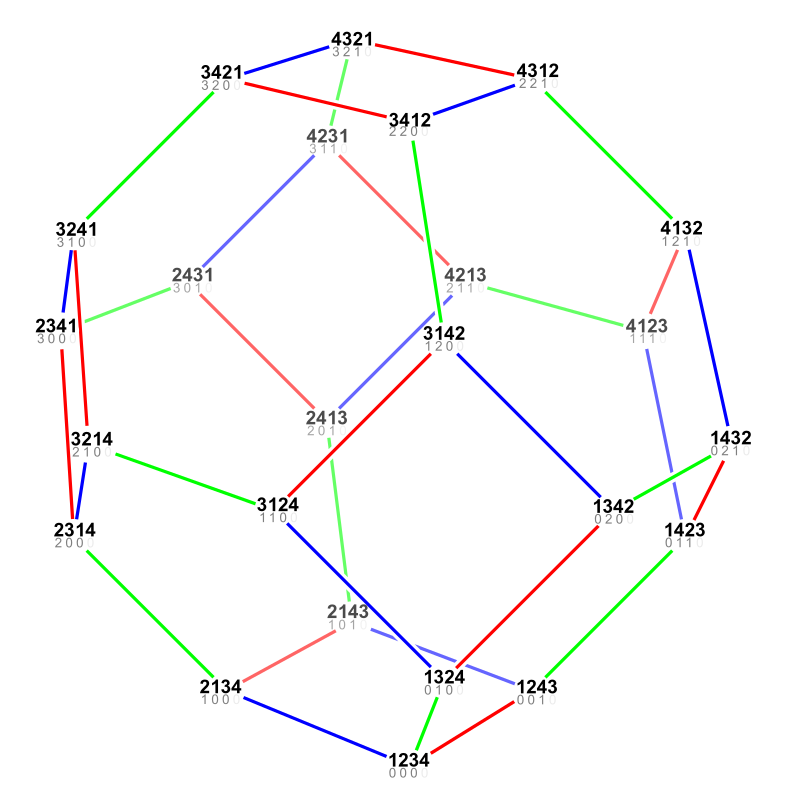
\includegraphics[scale=0.3]{img/permutohedron4.png}
    \end{figure}
By introducing equivalent definition of $Permutohedron$ it can be proved that every "permutation" is indeed vertex of Permutohedron and that there exists edge between
two vertices associated with two permutations $\sigma_1, \sigma_2$ if and only if there exists a transposition of two next elements  $\sigma_3 = (i $ $ i+1)$, $i=1,..n-1$ such that  $ \sigma_2 = \sigma_3 \circ \sigma_1$.
\newline 
It can be intuitively understood by the fact, that these are the closest neighbours in the standard Euclidian metric. 
\newline
Since we can look at  $n$-dimensional Permutohedron as graph, Main theorem in this paper is an algorithm for finding the shortest path between two vertices. 
\newline
It can be shown that
this problem is equivalent to sorting an array of length $n$ only by swapping consecutive elements. Therefore any algorithm providing that, can be used to find the shortest path. 
\newline
An array to be sorted that way, needs in edge case $\frac{n(n-1)}{2}2$ swaps - which is also the diameter of Permutohedron, therefore shown algorithm is the fastest possible if we want 
to find the shortest path.
\newline
If we only need a length of it, we can use approach similair to the merge sort algorithm, which can find an answer in $O(n\log(n))$ time
but the exact path cannot be found that way. 

\begin{thebibliography}{000}
    \bibitem{Convexity}
    Alexander Barvinok. \emph{A Course in Convexity} 
    \bibitem{Permuoahedron MIMUW}
    G. Lancia, P. Serafini. \emph{Compact Extended Linear Programming Models}
    
    \bibitem{Permutohedron v2}
    Micheal X. Goemans. \emph{Smallest Compact Forumlation for the Permutahedron}
\end{thebibliography}    
\end{document}